% !TeX program = pdflatex
\documentclass[border=6pt]{standalone}
\usepackage{tikz}
\usetikzlibrary{arrows.meta, positioning, calc}

\definecolor{MediumRed}{rgb}{0.925, 0.345, 0.345}
\definecolor{MediumGreen}{rgb}{0.37, 0.7, 0.66}
\definecolor{MediumBlue}{rgb}{0.015, 0.315, 0.45}
\definecolor{DarkBlue}{rgb}{0.05, 0.15, 0.35}

% 1. Define your text formatting macros here using \newcommand
\newcommand{\tit}{\sffamily\bfseries}
\newcommand{\con}{\scriptsize\color{MediumRed!60!black}}
\newcommand{\pro}{\scriptsize\color{MediumGreen!35!black}}

\begin{document}
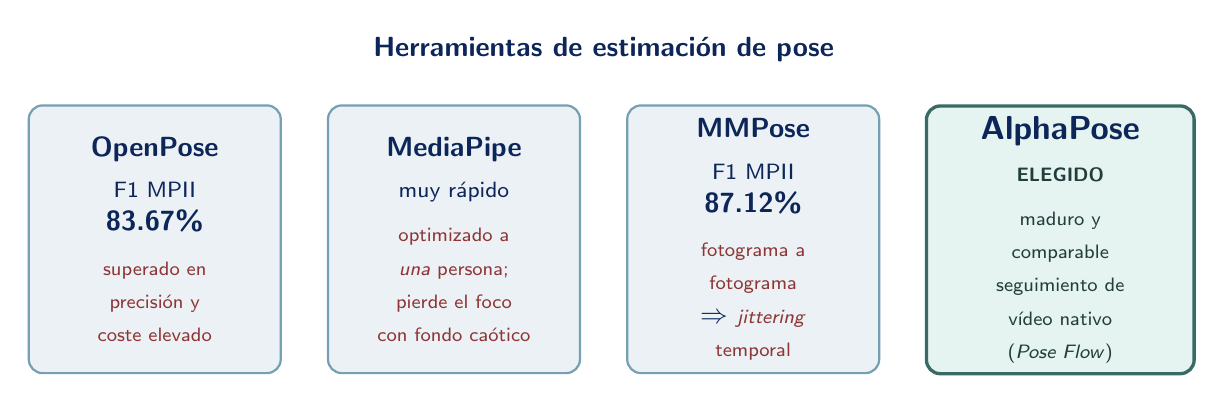
\begin{tikzpicture}[
    font=\sffamily,
    card/.style={draw=MediumBlue!55, thick, rounded corners=5pt, fill=MediumBlue!8,
        text=DarkBlue, align=center, minimum width=3.2cm, minimum height=3.4cm,
        anchor=north},
    win/.style={draw=MediumGreen!60!black, very thick, rounded corners=5pt,
        fill=MediumGreen!16, text=DarkBlue, align=center, minimum width=3.4cm,
        minimum height=3.4cm, anchor=north}
    % (Removed the old tit, con, and pro TikZ styles from here)
]

\node[card] (op) at (0,0)
    {\tit OpenPose\\[3pt]\footnotesize F1 MPII\\ \textbf{83.67\%}\\[4pt]
     \con superado en\\\con precisión y\\\con coste elevado};

\node[card] (mp) at (3.8,0)
    {\tit MediaPipe\\[3pt]\footnotesize muy rápido\\[4pt]
     \con optimizado a\\\con \emph{una} persona;\\\con pierde el foco\\\con con fondo caótico};

\node[card] (mm) at (7.6,0)
    {\tit MMPose\\[3pt]\footnotesize F1 MPII\\ \textbf{87.12\%}\\[4pt]
     \con fotograma a\\\con fotograma\\ $\Rightarrow$ \con \emph{jittering}\\\con temporal};

\node[win] (ap) at (11.5,0)
    {\tit\large AlphaPose\\[3pt]\pro \textbf{ELEGIDO}\\[4pt]
     \pro maduro y\\\pro comparable\\\pro seguimiento de\\\pro vídeo nativo\\\pro (\emph{Pose Flow})};

\node[font=\sffamily\bfseries, text=DarkBlue] at ($(op.north)!0.5!(mm.north)+(1.9,0.7)$)
    {\normalsize Herramientas de estimación de pose};

\end{tikzpicture}
\end{document}
